\section{Controllo centralizzato}

In alcuni casi il \textbf{controllo decentralizzato} a giunti indipendenti \textbf{può risultare inadeguato}. Questo accade, ad esempio, quando:
\begin{itemize}
	\item sono \textbf{richieste velocità operative elevate} $\implies$ le coppie di disturbo strutturato dipendenti dalla velocità (di Coriolis, centrifughe) influiscono pesantemente sul comportamento dei giunti
	\item i \textbf{motori sono ad azione diretta} $\implies$ a causa dell’assenza dei motoriduttori ($\mathbf{K}_r = \mathbf{I}$) non si beneficia di alcuna riduzione degli effetti non lineari e di accoppiamento fra i giunti
\end{itemize}
 
In tali casi gli effetti delle coppie di disturbo $\mathbf{d}$ possono determinare errori troppo elevati di inseguimento della traiettoria.
 
Poiché in questi casi non è possibile ridurre sufficientemente gli effetti indotti dalle coppie di disturbo $\mathbf{d}$, diventa conveniente cercare di eliminare direttamente tali coppie, ricorrendo ad una \textbf{strategia di controllo contenente termini non lineari di compensazione}.\\
Si parla di \textbf{controllo centralizzato} perché la coppia applicata a ciascun giunto risulta funzione anche delle variabili di posizione e velocità degli altri giunti, a differenza di quanto accade nel controllo a giunti indipendenti.
 
Negli schemi di controllo centralizzato il manipolatore è considerato come un \textbf{unico sistema MIMO}, con n ingressi (le coppie applicate ai giunti) e n uscite (le posizioni dei giunti) che interagiscono fra loro secondo relazioni non lineari. La \textbf{legge di controllo} centralizzato dovrà tenere conto del modello dinamico del manipolatore ed essere \textbf{non-lineare} (visto che il modello è non lineare).
 
 
 
\subsubsection{Idea principale}
Il principale approccio di controllo centralizzato è detto a \textbf{dinamica inversa}, perché la coppia di comando è ricavata dall’equazione dinamica del manipolatore a partire dalla conoscenza delle variabili giunto (posizioni e velocità), ovvero dalla risoluzione del problema della dinamica inversa.\\
Ovvero usando il modello dinamico:
\boldmath
$$
B(q)\ddot{q} + C(q, \dot{q})\dot{q} + F_v\dot{q} + g(q) = \tau
$$
\unboldmath

ci calcoliamo $\boldsymbol{\tau}$, che poi andiamo a fornire ai nostri attuatori, che quindi in questo caso saranno in modalità \textbf{torque-controlled}.




\subsubsection{Ora usiamo attuatori torque-controlled}
Come accennato in questo caso abbiamo bisogno di generatori di coppia.

Richiamando la forma semplificata del bilancio elettrico di armatura (\ref{eq:simplified_armature_electrical_balance}), possiamo scrivere:
$$
I_a = R_a^{-a}(V_a - K_\omega \omega_m) = R_a^{-1}(G_vV_c - K_\omega \omega_m)
$$
Dove l'ultima ugualianza deriva dall'amplificatore di potenza: $V_a = G_v V_c$.
Di conseguenza, ricordando (sempre al modello del motore: vedi fig. \ref{fig:electricactuator1}), che $\tau_m = K_t I_a$, possiamo scrivere:
$$
\tau = K_r \tau_m = K_r K_t I_a = K_r K_t R_a^{-1}(G_vV_c - K_\omega \omega_m)
$$
che si può notare essere uguale a (\ref{eq:torque_command}).

Visto che però vogliamo avere un motore torque-controlled (come possiamo ricordare) è necessario inserire la corrente in retroazione. Per magimagia (forse vedi sezione \ref{section:torque_generator}) diciamo che il termine con $K_\omega$ diventa trascurabile e quindi:
$$
I_a = R_a^{-1}(G_vV_c) = G_i V_c
$$
Di conseguenza
\boldmath
$$
\tau = K_r K_t G_i V_c = u
$$
\unboldmath
ove $\mathbf{u}$ è il vettore di comandi disponibili per il controllo.








\subsection{Controllo a dinamica inversa}
L’approccio di controllo a dinamica inversa è basato sull’idea di ottenere una \textbf{linearizzazione della dinamica del sistema per mezzo di una retroazione non lineare} degli stati tale da condurre ad un sistema lineare e disaccoppiato rispetto ad un nuovo vettore di accelerazioni di comando da progettare. Ovvero utilizzamo la tecnica nota come \textbf{feedback linearization}.

Prima di cominciare, per comodità definiamo il modello della dinamica come:
\boldmath
$$
B(q)\ddot{q} + n(q, \dot{q}) = \tau = u
$$
dove:
$$
n(q, \dot{q}) \triangleq C(q, \dot{q})\dot{q} + F_v\dot{q} + g(q)
$$
\unboldmath

Supponendo di poter calcolare esattamente $\mathbf{B(q)}$ e $\mathbf{n(q, \dot{q})}$, definiamo il nostro comando di controllo come
\boldmath
$$
u = B(q)y + n(q, \dot{q})
$$
questo perchè, così facendo, riusciamo ad ottenere una \textbf{linearizzazione esatta del sistema}:
\begin{gather*}
B(q)\ddot{q} + \cancel{n(q, \dot{q})} = \tau = u = B(q)y + \cancel{n(q, \dot{q})} \\
\Updownarrow \\
\cancel{B(q)}\ddot{q} = \cancel{B(q)}y \\
\Updownarrow \\
\ddot{q} = y
\end{gather*}
Il sistema risultante è costituito da n doppi integratori: la i-esima componente $y_i$ del nuovo comando influenza solo il comportamento della i-esima coordinata giunto $q_i$, che risulta indipendente dal moto degli altri giunti.


\begin{figure}[H]
	\centering
	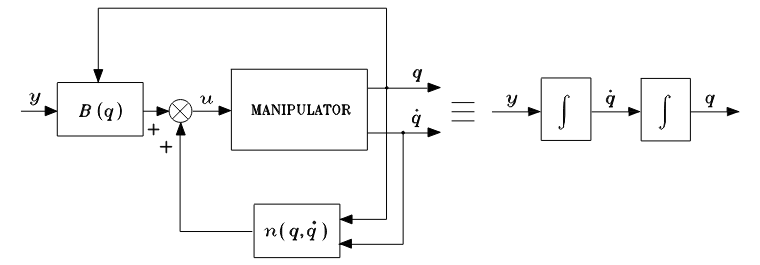
\includegraphics[width=0.8\linewidth]{images/centralized_control_1}
	\caption{Feedback linearization}
	\label{fig:centralizedcontrol1}
\end{figure}

La scelta più semplice per il nuovo comando $\mathbf{y}$ è data da una legge di \textbf{controllo di tipo PD}:
$$
y = -K_p q - K_D \dot{q} + r
$$

che quindi, sostituiendo a $\ddot{q} = y$, otteniamo il seguente sistema di equazioni del secondo ordine:
$$
\ddot{q} + K_p q + K_D \dot{q} = r
$$
asintoticamente stabile se le matrici $K_P$ e $K_D$ sono definite positive.
Scegliendo in particolare $K_P$ e $K_D$ diagonali, il sistema rimane disaccoppiato e ad ogni variabile giunto viene assegnata la dinamica corrispondente ai guadagni imposti con:
\unboldmath
$$
\mathbf{K_P} = diag\{\omega_{n1}^2, \ \dots, \ \omega_{nn}^2\}
\quad
\mathbf{K_D} = diag\{2\zeta\omega_{n1}, \ \dots, \ 2\zeta\omega_{nn}^2\}
$$



\hl{TODO DA SLIDE 12}


